\chapter{Sampling Plans}\label{Sampling Plans}


\begin{figure}[H]
    \centering
    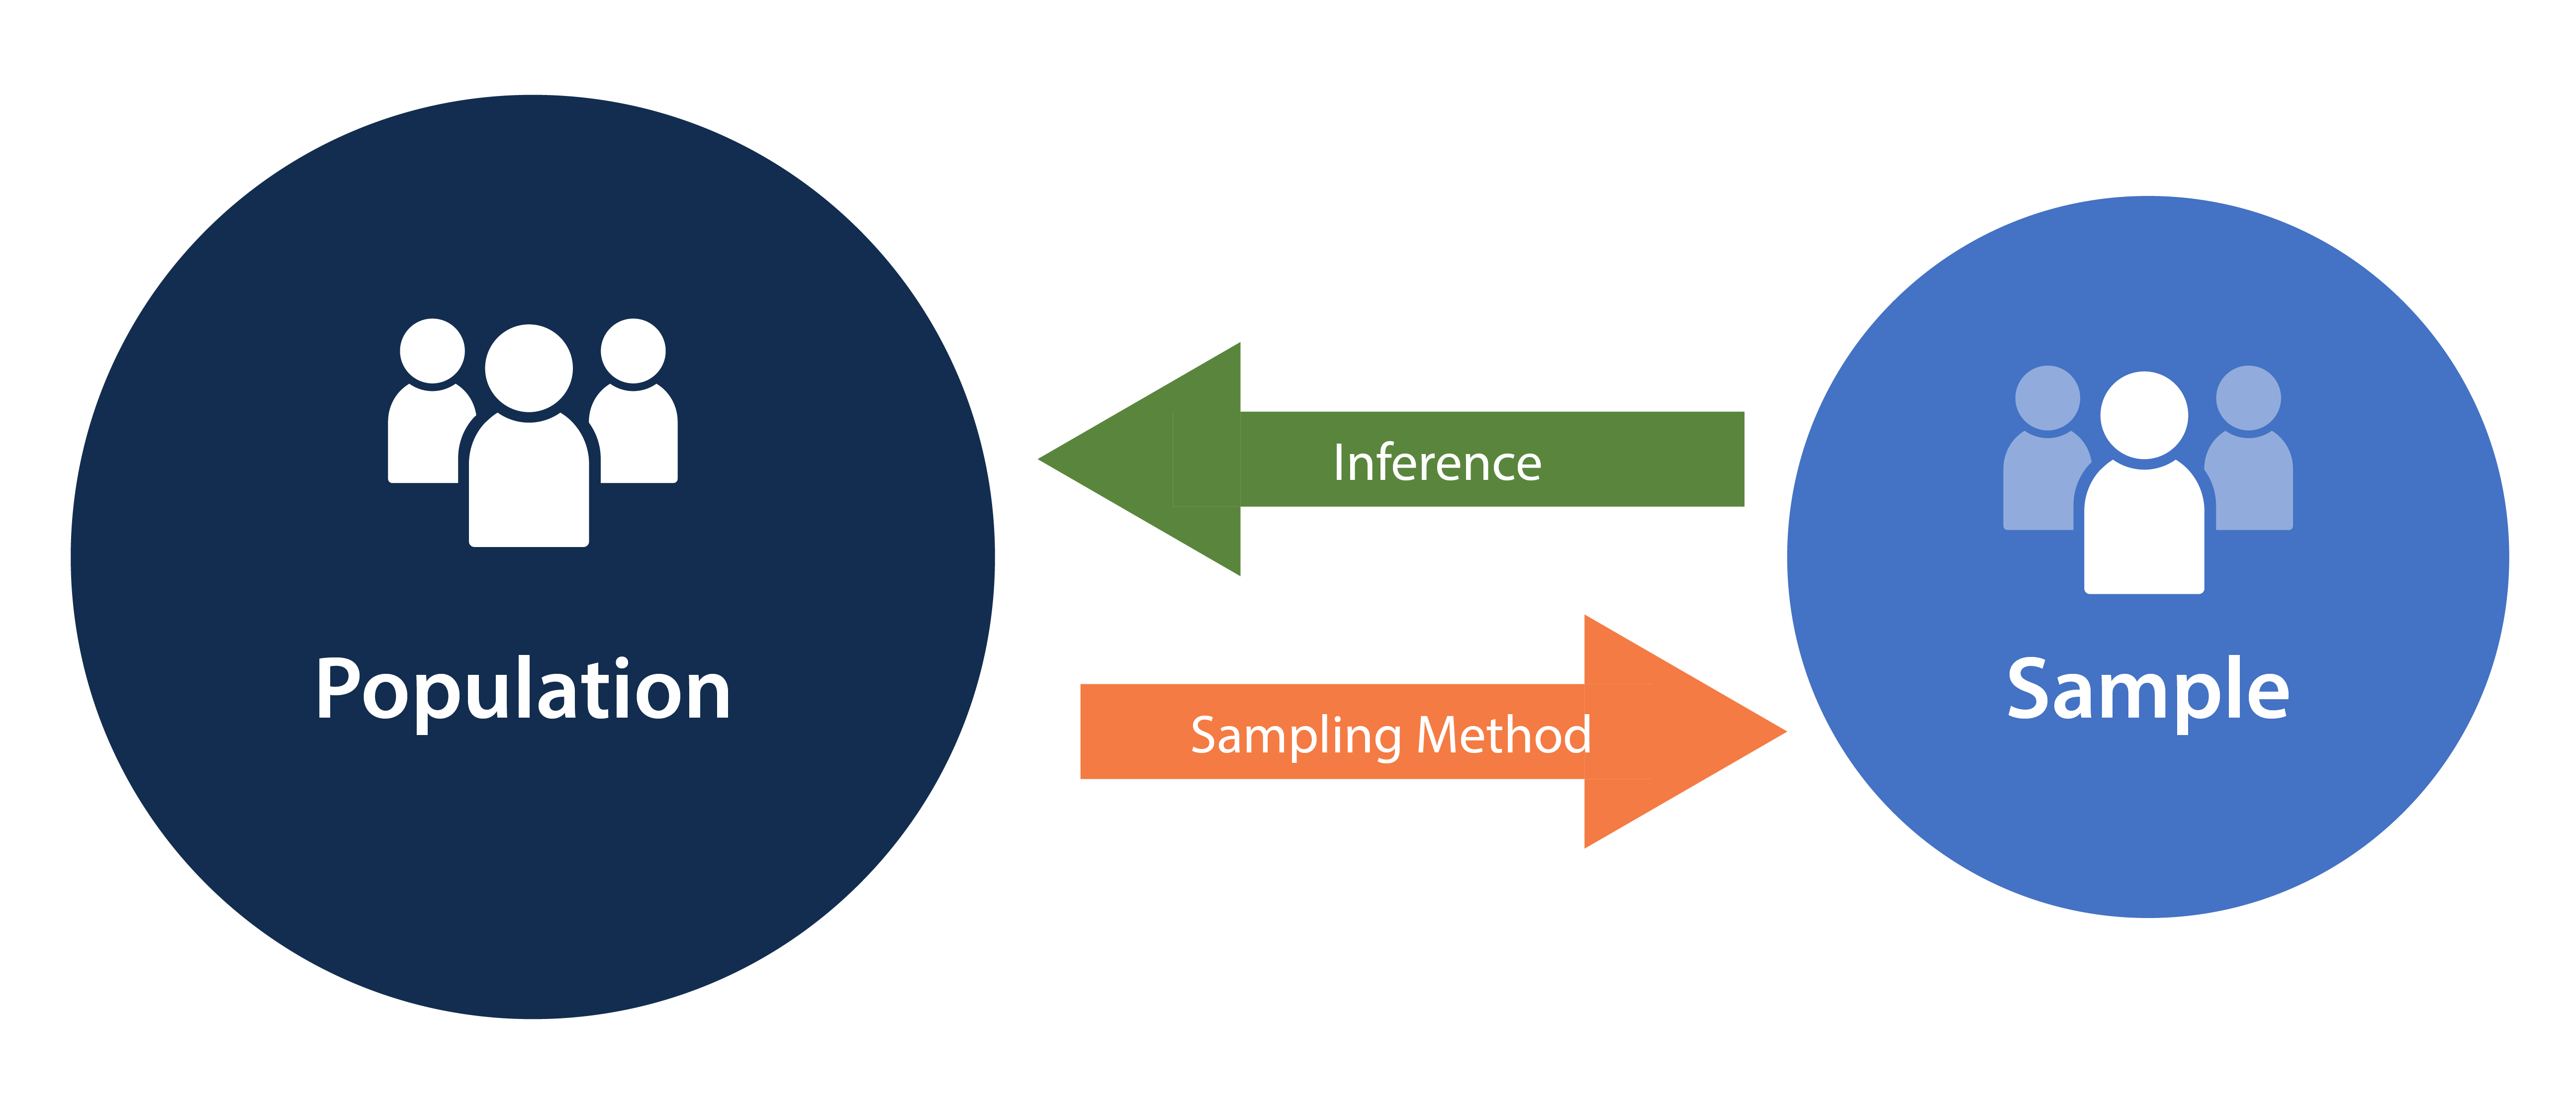
\includegraphics[
        width=0.5\linewidth, 
        height=5cm, 
        keepaspectratio
    ]{images/statistics/sampling-plan.png}

    \caption{Sampling Plan: Relation between Population and Sample}
\end{figure}


\begin{enumerate}
    \item \textbf{Statistical Inference}\label{Sampling Plans/Statistical Inference}: To extend your conclusions beyond the observed data. 
    The field of \textbf{inferential statistics} tries to use the information from a sample to make statements or decisions about the population of interest. 
    It takes into account the uncertainty that the information is coming from sampling and does not perfectly represent the population, since another sample would give different outcomes. 
    An important aspect of inferential statistics is estimation of the population parameters of interest.
    \hfill \cite{statistics/book/Statistics-for-Data-Scientists/Maurits-Kaptein}

    \item Sampling procedures are formal \textit{probabilistic approaches} to help collect units from the population for the sample.
    \hfill \cite{statistics/book/Statistics-for-Data-Scientists/Maurits-Kaptein}

    \item \textbf{Population}\label{Sampling Plans/Population}: The complete set of units that we would like to say something about is called the (target) population.
    \hfill \cite{statistics/book/Statistics-for-Data-Scientists/Maurits-Kaptein}
    \\
    In principle we would expect that a population is \textbf{always finite}, since an infinite number of units does not exist in real life. However, populations are often treated as infinite. One reason is that populations can be really really large.
    \hfill \cite{statistics/book/Statistics-for-Data-Scientists/Maurits-Kaptein}
    \\
    It is mathematically often more convenient (as we will see later) to assume that such a population is infinite.
    \hfill \cite{statistics/book/Statistics-for-Data-Scientists/Maurits-Kaptein}
    \\
    Properly defining or describing a population can be difficult. Furthermore, even if the population is established, measuring all units is often impossible or too elaborate. This means that information about the population can only be obtained by considering a subset of the population.
    \hfill \cite{statistics/book/Statistics-for-Data-Scientists/Maurits-Kaptein}

    \item \textbf{Sample}\label{Sampling Plans/Sample}: The set of units for which we have obtained data is referred to as the sample. 
    \hfill \cite{statistics/book/Statistics-for-Data-Scientists/Maurits-Kaptein}
    \\
    The sample is typically a subset of the population, although in theory the sample can form the whole population or the sample can contain units that are not from the target population. 
    \hfill \cite{statistics/book/Statistics-for-Data-Scientists/Maurits-Kaptein}

    \item \textbf{Representative Sample}\label{Sampling Plans/Representative Sample}:  A representative sample can be intuitively defined as a sample of units that has approximately the same distribution of characteristics as the population from which it was drawn.
    \hfill \cite{statistics/book/Statistics-for-Data-Scientists/Maurits-Kaptein}
    \\
    Representative sampling is also referred to as random or probability sampling.
    \hfill \cite{statistics/book/Statistics-for-Data-Scientists/Maurits-Kaptein}

    \item \textbf{Unit}\label{Sampling Plans/Unit}: A unit is usually a concrete or physical thing for which we would like to measure its characteristics.
    \hfill \cite{statistics/book/Statistics-for-Data-Scientists/Maurits-Kaptein}

    \item \textbf{Estimates}\label{Sampling Plans/Estimates}: In terms of statistical inference, the calculations on the sample data are referred to as estimates for the theoretical value in the whole population.
    \hfill \cite{statistics/book/Statistics-for-Data-Scientists/Maurits-Kaptein}

    \item \textbf{Estimators}\label{Sampling Plans/Estimators}: quantities that we compute using the data in our sample to say something about the population.
    \hfill \cite{statistics/book/Statistics-for-Data-Scientists/Maurits-Kaptein}

    \item \textbf{Realization}\label{Sampling Plans/realization}: The values in the sample are referred to as a realization from the population.
    \hfill \cite{statistics/book/Statistics-for-Data-Scientists/Maurits-Kaptein}

    %%%%%%%%%%%%%%%%%%%%%%%%%%%%%%%%%%%%%%%%%%%%%%%%%%%%%%%%%%%%%%%%%%%%%%%%%%%%%%
    \vspace{0.5cm}

    \item Reasons for sample instead of population:
    \begin{enumerate}
        \item In many applications we really can’t measure the complete population. For instance, one of the tests applied to aircraft engines is the “frozen bird test”. 
        \hfill \cite{statistics/book/Statistics-for-Data-Scientists/Maurits-Kaptein}

        \item Time, space, or budget restrictions often do not allow us to measure all units from a population.
        \hfill \cite{statistics/book/Statistics-for-Data-Scientists/Maurits-Kaptein}

        \item  Big data itself may be an argument for sampling. If we have a very large sample or we have been able to measure all units from the population, the resulting dataset can be so large that it becomes impossible to analyze the full data at one computer.
        \hfill \cite{statistics/book/Statistics-for-Data-Scientists/Maurits-Kaptein}
    \end{enumerate}

    \item A non-representative sample implies that we do not know the exact process by which units in the population became part of the sample.
    \hfill \cite{statistics/book/Statistics-for-Data-Scientists/Maurits-Kaptein}

    \item If we know which sampling procedure was applied to collect the units for the sample, we would also know how close the calculations or statistics would be to the theoretical value in the whole population.
    \hfill \cite{statistics/book/Statistics-for-Data-Scientists/Maurits-Kaptein}
    \\
    Thus the sampling procedure and the choice of calculation on the sample data (\\
    \nameref{Data/Describing Data/Central Tendency/(Arithmetic) mean or average}, \\
    \nameref{Data/Describing Data/Central Tendency/Median},\\
    \nameref{Data/Describing Data/Central Tendency/Quartiles/first quartile}, \\
    \nameref{Data/Describing Data/Central Tendency/Standard Deviation}\\
    etc.) would make statistical inference mathematically precise and it would therefore help us when making statements beyond the sample data.
    \hfill \cite{statistics/book/Statistics-for-Data-Scientists/Maurits-Kaptein}


\end{enumerate}

\section{Generic Formulation \cite{statistics/book/Statistics-for-Data-Scientists/Maurits-Kaptein}}

\begin{customArrayStretch}{1.3}
\begin{longtable}{>{\RaggedRight\arraybackslash}p{4cm} >{\centering\arraybackslash}p{0.5cm} p{10.5cm}}

\hhline{=:=:=} \endfirsthead
\hhline{=:=:=} \endhead
\hhline{=:=:=} \endfoot
\hhline{=:=:=} \endlastfoot


\textbf{Population Size} &
    $N$ &
    \hfill \cite{statistics/book/Statistics-for-Data-Scientists/Maurits-Kaptein}
    \\ \hline

\textbf{Sample Size} &
    $n$ &
    \begin{minipage}{10.3cm}
        \vspace{0.15cm}
        \begin{enumerate}
            \item $n \leq N$
            \hfill \cite{statistics/book/Statistics-for-Data-Scientists/Maurits-Kaptein}
            
        \end{enumerate}
        \vspace{0.15cm}
    \end{minipage} 
    \\ \hline

\textbf{Number of Possible Samples} &
    $K$ &
    \begin{minipage}{10.3cm}
        \vspace{0.15cm}
        \begin{enumerate}
            \item exact value of $K$ depends on the sampling plan
            \hfill \cite{statistics/book/Statistics-for-Data-Scientists/Maurits-Kaptein}
            
        \end{enumerate}
        \vspace{0.15cm}
    \end{minipage} 
    \\ \hline

\textbf{Population} &
    $\Omega$ &
    \begin{minipage}{10.3cm}
        \vspace{0.15cm}
        \begin{enumerate}
            \item $\Omega = \dCurlyBrac{1,2,\cdots,N}$
            \hfill \cite{statistics/book/Statistics-for-Data-Scientists/Maurits-Kaptein}
            
            \item $\Omega = \dbigcup_{k=1}^K S_k$
            \hfill \cite{statistics/book/Statistics-for-Data-Scientists/Maurits-Kaptein}
        \end{enumerate}
        \vspace{0.15cm}
    \end{minipage} 
    \\ \hline


\textbf{Sample} &
    $S_k$ &
    \begin{minipage}{10.3cm}
        \vspace{0.15cm}
        \begin{enumerate}
            \item Subset of Population
            \hfill \cite{statistics/book/Statistics-for-Data-Scientists/Maurits-Kaptein}
            
            \item $k \in \dCurlyBrac{1,2,\cdots, K}$
            \hfill \cite{statistics/book/Statistics-for-Data-Scientists/Maurits-Kaptein}
            
            \item $S_k = \dCurlyBrac{i_1,i_2,\cdots,i_n}$  ($i_h \in \dParenBrac{1,\cdots,N}$)
            \hfill \cite{statistics/book/Statistics-for-Data-Scientists/Maurits-Kaptein}
            \\
            ($n$ unique units, $h \neq l \Rightarrow i_h \neq i_l$)
            \hfill \cite{statistics/book/Statistics-for-Data-Scientists/Maurits-Kaptein}
            
            \item $S_k \subset \Omega \hspace{2cm} \forall\  k \in \dParenBrac{1,\cdots,K}$
            \hfill \cite{statistics/book/Statistics-for-Data-Scientists/Maurits-Kaptein}


            \item Each subset is unique: $k\neq l \Rightarrow S_k \neq S_l$
            \hfill \cite{statistics/book/Statistics-for-Data-Scientists/Maurits-Kaptein}

            \item Subsets may overlap: $S_k \ \cap\ S_l \neq \phi$
            \hfill \cite{statistics/book/Statistics-for-Data-Scientists/Maurits-Kaptein}
        \end{enumerate}
        \vspace{0.15cm}
    \end{minipage} 
    \\ \hline


\textbf{Unit} &
    $i$ &
    \hfill \cite{statistics/book/Statistics-for-Data-Scientists/Maurits-Kaptein}
    \\ \hline

\textbf{Unit's  theoretical value} &
    $x_i$ &
    \hfill \cite{statistics/book/Statistics-for-Data-Scientists/Maurits-Kaptein}
    \\ \hline

\textbf{Sample probability} &
    $\pi_k$ &
    \begin{minipage}{10.3cm}
        \vspace{0.15cm}
        \begin{enumerate}
            \item each subset $S_k$ is attached a probability $\pi_k$
            \hfill \cite{statistics/book/Statistics-for-Data-Scientists/Maurits-Kaptein}
            
            \item $\pi_k > 0 \hspace{2cm}  k \in \dCurlyBrac{1,\cdots,K}$
            \hfill \cite{statistics/book/Statistics-for-Data-Scientists/Maurits-Kaptein}
            
            \item $\dsum_{k=1}^K \pi_k = 1$
            \hfill \cite{statistics/book/Statistics-for-Data-Scientists/Maurits-Kaptein}
        \end{enumerate}
        \vspace{0.15cm}
    \end{minipage} 
    \\ \hline


\textbf{Unit Probability} &
    $p_i$ &
    \begin{minipage}{10.3cm}
        \vspace{0.15cm}
        \begin{enumerate}
            \item Probability of each unit in population
            \hfill \cite{statistics/book/Statistics-for-Data-Scientists/Maurits-Kaptein}
            
            \item $p_i > 0 \hspace{2cm} \ i \in \dCurlyBrac{1,\cdots,N}$
            \hfill \cite{statistics/book/Statistics-for-Data-Scientists/Maurits-Kaptein}

            \item $\dsum_{i=1}^N p_i \neq 1$ since samples overlap
            \hfill \cite{statistics/book/Statistics-for-Data-Scientists/Maurits-Kaptein}

            \item the probabilities are \textbf{not} always the same for each unit.
            \hfill \cite{statistics/book/Statistics-for-Data-Scientists/Maurits-Kaptein}

        \end{enumerate}
        \vspace{0.15cm}
    \end{minipage} 
    \\ \hline


\textbf{Population Parameter} &
    $\theta$ &
    \begin{minipage}{10.3cm}
        \vspace{0.15cm}
        \begin{enumerate}
            \item $\theta \equiv \theta(\mathbf{x})$ where $\mathbf{x} = \dParenBrac{x_1, x_2, \cdots, x_N}$
            \hfill \cite{statistics/book/Statistics-for-Data-Scientists/Maurits-Kaptein}
            
        \end{enumerate}
        \vspace{0.15cm}
    \end{minipage} 
    \\ \hline


\textbf{Observations} &
    $\mathbf{x}_k^\top$ &
    \begin{minipage}{10.3cm}
        \vspace{0.15cm}
        \begin{enumerate}
            \item $\mathbf{x}_k^\top = \dParenBrac{x_{i_1}, x_{i_2}, \cdots, x_{i_n}}$
            \hfill \cite{statistics/book/Statistics-for-Data-Scientists/Maurits-Kaptein}

            \item Observed with every sample $S_k$
            \hfill \cite{statistics/book/Statistics-for-Data-Scientists/Maurits-Kaptein}
        \end{enumerate}
        \vspace{0.15cm}
    \end{minipage} 
    \\ \hline

\textbf{Descriptive Statistic/ Estimate} &
    $\hat{\theta}_k$ &
    \begin{minipage}{10.3cm}
        \vspace{0.15cm}
        \begin{enumerate}
            \item $\hat{\theta}_k = T(\mathbf{x}_k)$
            \hfill \cite{statistics/book/Statistics-for-Data-Scientists/Maurits-Kaptein}

            \item Computed based on the observed data.
            \hfill \cite{statistics/book/Statistics-for-Data-Scientists/Maurits-Kaptein}

            \item used as an \textit{estimate} for the population parameter $\theta$
            \hfill \cite{statistics/book/Statistics-for-Data-Scientists/Maurits-Kaptein}
            
        \end{enumerate}
        \vspace{0.15cm}
    \end{minipage} 
    \\ \hline

\textbf{Estimator} &
    $T(\cdot)$ &
    \begin{minipage}{10.3cm}
        \vspace{0.15cm}
        \begin{enumerate}
            \item It is a function applied to the observed data (i.e., some calculation procedure). 
            \hfill \cite{statistics/book/Statistics-for-Data-Scientists/Maurits-Kaptein}

            \item In many cases the function $T$ is identical to the calculation $\theta$ at the population level, but alternative functions may be used depending on the sampling plan.
            \hfill \cite{statistics/book/Statistics-for-Data-Scientists/Maurits-Kaptein}

            \item \textbf{Example}: For estimating population mean, $\bar{x}_k$ can be used as $T$ 
            \hfill \cite{statistics/book/Statistics-for-Data-Scientists/Maurits-Kaptein}
        \end{enumerate}
        \vspace{0.15cm}
    \end{minipage} 
    \\ \hline

\textbf{Expected Population Parameter} &
    $\mathbb{E}(T)$ &
    \begin{minipage}{10.3cm}
        \vspace{0.15cm}
        \begin{enumerate}
            \item $
                \mathbb{E}(T)
                = \dsum_{k=1}^{K} \hat{\theta}_k \pi_k
            $
            \hfill \cite{statistics/book/Statistics-for-Data-Scientists/Maurits-Kaptein}

            \item $
                \mathbb{E}(cT) = c\ \mathbb{E}(T)
                \hspace{1cm} \forall\  c \in \mbbR
            $
            \hfill \cite{statistics/book/Statistics-for-Data-Scientists/Maurits-Kaptein}

        \end{enumerate}
        \vspace{0.15cm}
    \end{minipage} 
    \\ \hline


\textbf{Weighted Average} &
    $\bar{x}_{w,k}$ &
    \begin{minipage}{10.3cm}
        \vspace{0.15cm}
        \begin{enumerate}
            \item $
                \bar{x}_{w,k}
                = \dsum_{i \in S_k} w_{ik}x_i
            $
            \hfill \cite{statistics/book/Statistics-for-Data-Scientists/Maurits-Kaptein}

            \item $
                \dsum_{i \in S_k} w_{ik} = 1
            $
            \hfill \cite{statistics/book/Statistics-for-Data-Scientists/Maurits-Kaptein}

            \item If every observation has the same weight, we obtain the arithmetic average $\bar{x}_k = \dfrac{1}{n} \dsum_{i \in S_k} x_i$
            \hfill \cite{statistics/book/Statistics-for-Data-Scientists/Maurits-Kaptein}

        \end{enumerate}
        \vspace{0.15cm}
    \end{minipage} 
    \\ \hline


\end{longtable}
\end{customArrayStretch}


\begin{enumerate}
    \item The set of samples $S_1, S_2,\cdots, S_K$ with their probabilities $\pi_1, \pi_2, \pi_3,\cdots,\pi_K$ is referred to as a \textbf{sampling plan}.
    \hfill \cite{statistics/book/Statistics-for-Data-Scientists/Maurits-Kaptein}

    \item The sampling plan contains all the information necessary to analyze the quality of a sampling procedure.
    \hfill \cite{statistics/book/Statistics-for-Data-Scientists/Maurits-Kaptein}

    \item \textbf{Population Mean}: \hspace{2cm} $
        \mu
        = \dfrac{1}{N}\dsum_{i=1}^N x_i
    $
    \hfill \cite{statistics/book/Statistics-for-Data-Scientists/Maurits-Kaptein}

    \item \textbf{Population Variance}: \hspace{2cm} $
        \sigma^2
        = \dfrac{1}{N}\dsum_{i=1}^N (x_i - \mu)^2
    $
    \hfill \cite{statistics/book/Statistics-for-Data-Scientists/Maurits-Kaptein}

    \item In general, the value $\hat{\theta}_k$ can be considered an estimate of the population parameter $\theta$ when sample $S_k$ would be collected. 
    \hfill \cite{statistics/book/Statistics-for-Data-Scientists/Maurits-Kaptein}
    
    \item The estimate $\hat{\theta}_k$ will most likely be different from the population parameter $\theta$, because the sample is just a subset of the population. 
    \hfill \cite{statistics/book/Statistics-for-Data-Scientists/Maurits-Kaptein}

    
\end{enumerate}
















\clearpage
\section{Measures of closeness}\label{Sampling Plans/Measures of closeness}


\begin{figure}[H]
    \centering
    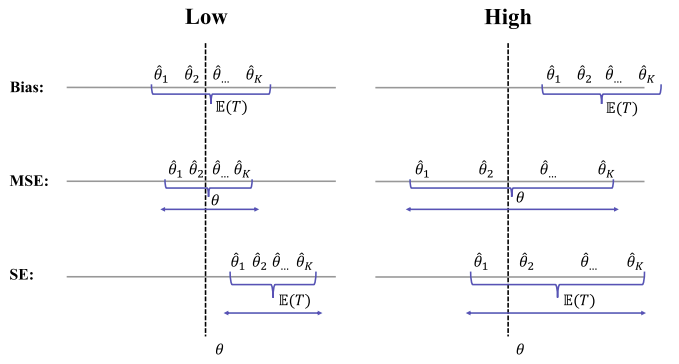
\includegraphics[
        width=0.7\linewidth, 
        height=6cm,
        keepaspectratio,
    ]{images/statistics/bias-se-mse-visual.png}
    \caption{Visual Representation of Bias, MSE and SE}
\end{figure}


\subsection{Bias}\label{Sampling Plans/Measures of closeness/Bias}

\hfill 
$
    bias
    = \dParenBrac{\dsum_{k=1}^{K} \hat{\theta}_k \pi_k} - \theta
    = \mathbb{E}(T) - \theta
$
\hfill \cite{statistics/book/Statistics-for-Data-Scientists/Maurits-Kaptein}

\vspace{0.5cm}

\begin{enumerate}
    \item The bias is the difference between the weighted average - over all possible $K$ samples - of the sample estimate $\hat{\theta}_k$'s and the true population parameter $\theta$.
    \hfill \cite{statistics/book/Statistics-for-Data-Scientists/Maurits-Kaptein}

    \item The weights in this weighted average are provided by the probabilities $\pi_k$.
    \hfill \cite{statistics/book/Statistics-for-Data-Scientists/Maurits-Kaptein}

    \item  If the bias of an estimator is \textbf{zero}, this means that, if we repeatedly take samples using our sampling plan and repeatedly compute our statistic of interest, the average over all of those statistics is equal to the true population parameter. 
    \hfill \cite{statistics/book/Statistics-for-Data-Scientists/Maurits-Kaptein}
    \\
    If the bias is \textbf{zero}, the estimator, under the sampling plan that is being evaluated, is said to be \textbf{unbiased}.
    \hfill \cite{statistics/book/Statistics-for-Data-Scientists/Maurits-Kaptein}

    \item The bias of an estimator is thus the difference between this estimator’s expected value and the true population value.
    \hfill \cite{statistics/book/Statistics-for-Data-Scientists/Maurits-Kaptein}

    \item A small bias of an estimator under a sampling plan does \textbf{not} guarantee that individual sample results $\hat{\theta}_k$ are actually close to the population parameter $\theta$; it just states that they are close on average, if we were to sample over and over again.
    \hfill \cite{statistics/book/Statistics-for-Data-Scientists/Maurits-Kaptein}

    \item If the bias is small, $\mathbb{E}(T)$ is close to the parameter value $\theta$.\\
    If the bias is large, $\mathbb{E}(T)$ is \textbf{not} close to $\theta$
    \hfill \cite{statistics/book/Statistics-for-Data-Scientists/Maurits-Kaptein}

    \item If the sampling plan is unbiased and thus $\mathbb{E}(T) = \theta$, the RMSE and the SE are identical.
    \hfill \cite{statistics/book/Statistics-for-Data-Scientists/Maurits-Kaptein}

    
\end{enumerate}









\subsection{Mean Square Error (MSE)}\label{Sampling Plans/Measures of closeness/Mean Square Error (MSE)}

\hfill
$
    MSE 
    = \dsum_{k=1}^{K} \dParenBrac{\hat{\theta}_k - \theta}^2 \pi_k
$
\hfill \cite{statistics/book/Statistics-for-Data-Scientists/Maurits-Kaptein}


\begin{enumerate}
    \item To capture the variability in the sample results $\hat{\theta}_1, \hat{\theta}_2,..., \hat{\theta}_K$ with respect to the true value $\theta$, we use the so-called mean squared error (MSE).
    \hfill \cite{statistics/book/Statistics-for-Data-Scientists/Maurits-Kaptein}

    \item The MSE measures the weighted average squared distance of the sample results $\hat{\theta}_1, \hat{\theta}_2,..., \hat{\theta}_K$ from the population parameter $\theta$.
    \hfill \cite{statistics/book/Statistics-for-Data-Scientists/Maurits-Kaptein}

    \item The weights are determined by the sampling probabilities. 
    \hfill \cite{statistics/book/Statistics-for-Data-Scientists/Maurits-Kaptein}

    \item The smaller the MSE the better the sampling plan. 
    \hfill \cite{statistics/book/Statistics-for-Data-Scientists/Maurits-Kaptein}

    \item If the MSE is small, the variability of the $\hat{\theta}_k$'s around $\theta$ is small, \\
    while if the MSE is large, the variability around $\theta$ is large.
    \hfill \cite{statistics/book/Statistics-for-Data-Scientists/Maurits-Kaptein}
\end{enumerate}







\subsection{Root Mean Square Error (RMSE)}\label{Sampling Plans/Measures of closeness/Root Mean Square Error (RMSE)}


\hfill
$
    RMSE 
    = \sqrt{MSE} 
    = \sqrt{{SE}^2 + \dParenBrac{\mathbb{E}(T) - \theta}^2}
$
\hfill \cite{statistics/book/Statistics-for-Data-Scientists/Maurits-Kaptein}






\subsection{Standard Error (SE)}\label{Sampling Plans/Measures of closeness/Standard Error (SE)}


\hfill
$
    SE = \sqrt{
        \dsum_{k=1}^{K} \dParenBrac{
            \hat{\theta}_k - \mathbb{E}(T)
        }^2
        \pi_k
    }
$
\hfill \cite{statistics/book/Statistics-for-Data-Scientists/Maurits-Kaptein}


\begin{enumerate}
    \item It represents the variability of the sampling plan with respect to the expected population parameter $\mathbb{E}(T)$ instead of using the true population parameter $\theta$.
    \hfill \cite{statistics/book/Statistics-for-Data-Scientists/Maurits-Kaptein}

    \item Standard error of an estimator is used as a measure to represent our uncertainty regarding an estimate.
    \hfill \cite{statistics/book/Statistics-for-Data-Scientists/Maurits-Kaptein}

    \item If the SE is small, the variability of the $\hat{\theta}_k$’s around $\mathbb{E}(T)$ is small. 
    \hfill \cite{statistics/book/Statistics-for-Data-Scientists/Maurits-Kaptein}

    \item $SE(cT ) = c\ SE(T) \hspace{2cm} \forall\  c \in \mbbR$
    \hfill \cite{statistics/book/Statistics-for-Data-Scientists/Maurits-Kaptein}
\end{enumerate}








\section{Types of Samplings}

\begin{enumerate}

\item \textbf{Non-representative Sampling} \label{Sampling Plans/Non-representative Sampling}
\hfill \cite{statistics/book/Statistics-for-Data-Scientists/Maurits-Kaptein}

    \begin{enumerate}
        \item Although these sampling methods are frequently in use, it is strongly recommended not to apply these methods, unless knowledge is available on how to adjust or correct the sample for inferential purposes.
        \hfill \cite{statistics/book/Statistics-for-Data-Scientists/Maurits-Kaptein}
    
        \item These have the risk that some units are much more likely to be included in the sample than others, which can make statistics computed on the sample data bad estimates for the population parameters of interest.
        \hfill \cite{statistics/book/Statistics-for-Data-Scientists/Maurits-Kaptein}
    
        \item With non-representative sampling some units are not only more likely to be included in the sample, we also do not actually know how likely units were included. 
        \hfill \cite{statistics/book/Statistics-for-Data-Scientists/Maurits-Kaptein}
    
        \item Even if we wanted to, we could not control for these systematic differences between units.
        \hfill \cite{statistics/book/Statistics-for-Data-Scientists/Maurits-Kaptein}
    \end{enumerate}

    \vspace{0.2cm}
    \textbf{SEE}:
    \begin{enumerate}
        \item \fullref{Sampling Plans/Non-representative Sampling/Convenience Sampling}
        \item \fullref{Sampling Plans/Non-representative Sampling/Haphazard Sampling}
        \item \fullref{Sampling Plans/Non-representative Sampling/Purposive Sampling or Judgmental Sampling}
    \end{enumerate}


\item \textbf{Representative Sampling} \label{Sampling Plans/Representative Sampling}
\hfill \cite{statistics/book/Statistics-for-Data-Scientists/Maurits-Kaptein}
    \begin{enumerate}
        \item We sample units in such a way that we do know how likely units are to be included in the sample (even if they will be different from unit to unit).
        \hfill \cite{statistics/book/Statistics-for-Data-Scientists/Maurits-Kaptein}
    
        \item Random sampling is a sampling method that uses a random mechanism. 
        \hfill \cite{statistics/book/Statistics-for-Data-Scientists/Maurits-Kaptein}
    
        \begin{enumerate}
            \item The probability of each unit in the population of becoming part of the sample is both positive and known.
            \hfill \cite{statistics/book/Statistics-for-Data-Scientists/Maurits-Kaptein}
        \end{enumerate}
    \end{enumerate}

    \vspace{0.2cm}
    \textbf{SEE}:
    \begin{enumerate}
        \item \fullref{Sampling Plans/Representative Sampling/Simple Random Sampling}
        \item \fullref{Sampling Plans/Representative Sampling/Systematic Sampling}
        \item \fullref{Sampling Plans/Representative Sampling/Stratified Sampling}
        \item \fullref{Sampling Plans/Representative Sampling/Cluster Sampling}
    \end{enumerate}
\end{enumerate}

\clearpage
\section{Convenience Sampling \cite{statistics/book/Statistics-for-Data-Scientists/Maurits-Kaptein}}\label{Sampling Plans/Non-representative Sampling/Convenience Sampling}

\begin{enumerate}
    \item Convenience sampling collects only units from the population that can be easily obtained.
    \hfill \cite{statistics/book/Statistics-for-Data-Scientists/Maurits-Kaptein}

    \item This may provide a biased sample, as it represents only one small part or time window of the whole processing window for a batch of products. The term \textbf{bias}\label{Sampling Plans/Non-representative Sampling/Convenience Sampling/bias} indicates that we obtain the value of interest with a systematic mistake.
    \hfill \cite{statistics/book/Statistics-for-Data-Scientists/Maurits-Kaptein}

    \item  Convenience sampling is often justified by using the argument of population homogeneity. This insinuates that either the population units are not truly different or the process produces the population of units in random order. 
    \hfill \cite{statistics/book/Statistics-for-Data-Scientists/Maurits-Kaptein}
\end{enumerate}


\section{Haphazard Sampling \cite{statistics/book/Statistics-for-Data-Scientists/Maurits-Kaptein}}\label{Sampling Plans/Non-representative Sampling/Haphazard Sampling}

\begin{enumerate}
    \item Haphazard sampling is often believed to be an excellent way of collecting samples, because it gives a feeling or the impression that each unit was collected completely at random.
    \hfill \cite{statistics/book/Statistics-for-Data-Scientists/Maurits-Kaptein}

    \item Despite the feeling of randomness when performing haphazard sampling, often the resulting sample is not truly random.
    \hfill \cite{statistics/book/Statistics-for-Data-Scientists/Maurits-Kaptein}
\end{enumerate}

\section{Purposive Sampling/ Judgmental Sampling \cite{statistics/book/Statistics-for-Data-Scientists/Maurits-Kaptein}}\label{Sampling Plans/Non-representative Sampling/Purposive Sampling or Judgmental Sampling}

\begin{enumerate}
    \item Purposive sampling or judgmental sampling tries to sample units for a specific purpose.
    \hfill \cite{statistics/book/Statistics-for-Data-Scientists/Maurits-Kaptein}

    \item This means that the collection of units is focused on one or more particular characteristics and hence it implies that only units that are more alike are sampled.
    \hfill \cite{statistics/book/Statistics-for-Data-Scientists/Maurits-Kaptein}

    \item This way of sampling is strongly related to the definition of the population, since deliberately excluding units from the sample is analogous to limiting the population of interest.
    \hfill \cite{statistics/book/Statistics-for-Data-Scientists/Maurits-Kaptein}

    \item Purposive sampling may be useful, but it is limited since it does not allow us in general to make statements about the whole population, and at best only about a limited part of the population (although we may not be sure either).
    \hfill \cite{statistics/book/Statistics-for-Data-Scientists/Maurits-Kaptein}

    \item It does most likely produce a biased sample with respect to the complete population.
    \hfill \cite{statistics/book/Statistics-for-Data-Scientists/Maurits-Kaptein}
\end{enumerate}


\clearpage
\section{Simple Random Sampling \cite{statistics/book/Statistics-for-Data-Scientists/Maurits-Kaptein}}\label{Sampling Plans/Representative Sampling/Simple Random Sampling}

\begin{table}[H]
    \centering
    \begin{tabular}{l l}
        $N$ & population size \\
        $n$ & sample size \\
        $K$ & number of possible samples \\
        $k$ & sample index ($ k \in \dParenBrac{1,\cdots,K}$) \\
        $S_k$ & sample\\
    \end{tabular}
\end{table}

\begin{enumerate}
    \item Implicitly assume that there is no particular group structure present in the population.
    \hfill \cite{statistics/book/Statistics-for-Data-Scientists/Maurits-Kaptein}

    \item Simple random sampling is a way of collecting samples such that each unit from the population has the exact same probability of becoming part of the sample.
    \hfill \cite{statistics/book/Statistics-for-Data-Scientists/Maurits-Kaptein}


    \item Simple random sampling is a conceptually easy method of forming random samples but it can prove hard in practice.
    \hfill \cite{statistics/book/Statistics-for-Data-Scientists/Maurits-Kaptein}

    \item Simple random sampling is frequently combined with other choices or settings (see stratified and cluster sampling).
    \hfill \cite{statistics/book/Statistics-for-Data-Scientists/Maurits-Kaptein}

    \item Number of unique samples $
        = K
        = \dfrac{N!}{n!(N-n)!}
    $
    \hfill \cite{statistics/book/Statistics-for-Data-Scientists/Maurits-Kaptein}

    \item the probability of collecting sample $S_k$, using sequential sampling $
        = \dfrac{1}{K}
        = \dfrac{n!(N-n)!}{N!}
    $
    \hfill \cite{statistics/book/Statistics-for-Data-Scientists/Maurits-Kaptein}

    \item The probability that a specific unit is part of the sample $
        = \dfrac{n}{N}
    $
    \hfill \cite{statistics/book/Statistics-for-Data-Scientists/Maurits-Kaptein}

    \item The probability that a specific unit is \textbf{not} contained in the sample $
        = 1 - \dfrac{n}{N}
        = \dfrac{N-n}{N}
    $
    \hfill \cite{statistics/book/Statistics-for-Data-Scientists/Maurits-Kaptein}

    \item The number of samples that does \textbf{not} contain a specific unit $
        = \dfrac{(N - 1)!}{n!(N - 1 - n)!}
    $
    \hfill \cite{statistics/book/Statistics-for-Data-Scientists/Maurits-Kaptein}

    \item Number of samples that contain certain unit $i$ = $\dfrac{nK}{N}$
    \hfill \cite{statistics/book/Statistics-for-Data-Scientists/Maurits-Kaptein}
    \\
    $
        \Rightarrow
        \dsum_{k=1}^{K}\ \dsum_{i \in S_k} x_i
        = \dfrac{nK}{N}\dsum_{i=1}^{N} x_i
    $
    \hfill \cite{statistics/book/Statistics-for-Data-Scientists/Maurits-Kaptein}

    \item Population Variance: $
        \sigma^2
        = \dfrac{1}{N} \dsum_{i=1}^N (x_i-\mu)^2
    $
    \hfill \cite{statistics/book/Statistics-for-Data-Scientists/Maurits-Kaptein}

    \item \textbf{Disadvantage}: When the numbers of units across these subpopulations are (substantially) different, simple random may not collect units from each subgroup.
    \hfill \cite{statistics/book/Statistics-for-Data-Scientists/Maurits-Kaptein}

\end{enumerate}

\vspace{0.5cm}
\textbf{Example}:
\begin{enumerate}
    \item[] $N = 20,\ n = 5$

    \item[] $K = \dfrac{20!}{5!\cdot 15!}=15504$


\end{enumerate}


\subsection{Estimation for population mean}
\begin{enumerate}
    \item Estimator: $
        T
        = \bar{x}
        = \dfrac{1}{n} \dsum_{i=1}^n x_i
    $
    \hfill \cite{statistics/book/Statistics-for-Data-Scientists/Maurits-Kaptein}

    \item Bias: $0$
    \hfill \cite{statistics/book/Statistics-for-Data-Scientists/Maurits-Kaptein}

    \item $
        MSE(\bar{x}_k)
        = \dfrac{\sigma^2 }{n}
        \dParenBrac{\dfrac{N}{N-1}}
        \dParenBrac{1-\dfrac{n}{N}}
        = \dfrac{\sigma^2\ (N-n)}{n\ (N-1)}
    $
    \hfill \cite{statistics/book/Statistics-for-Data-Scientists/Maurits-Kaptein}
    \\
    MSE shows that it becomes equal to zero when the sample size $n$ becomes equal to the population size $N$.
    \hfill \cite{statistics/book/Statistics-for-Data-Scientists/Maurits-Kaptein}
    \\
    The MSE will not become zero when the estimator is biased, even if the sample size is equal to the population size.
    \hfill \cite{statistics/book/Statistics-for-Data-Scientists/Maurits-Kaptein}


    \item $
        \mathbb{E}[T]
        = \dfrac{1}{K}\dsum_{k=1}^{K} \bar{x}_k
        = \dfrac{1}{nK}\dsum_{k=1}^{K}\ \dsum_{i \in S_k} x_i
        = \dfrac{1}{N}\dsum_{i=1}^{N} x_i
        = \mu
    $
    \hfill \cite{statistics/book/Statistics-for-Data-Scientists/Maurits-Kaptein}
\end{enumerate}


\subsection{Estimation of the sample MSE}

\begin{enumerate}
    \item unbiased estimator for $\sigma^2$: \\
    $
       \hat{\sigma}^2 = \dfrac{N - 1}{N}\ s^2_k
    $
    \hfill
    $
        \dParenBrac{\
            s^2_k = \dfrac{1}{n - 1} \dsum_{i\ \in\ S_k} (x_i - \bar{x}_k )^2
        \ }
    $
    \hfill \cite{statistics/book/Statistics-for-Data-Scientists/Maurits-Kaptein}

    \item $
        \hat{MSE}(\bar{x}_k)
        = \dfrac{N - n}{N n}\ s^2_k
    $
    \hfill \cite{statistics/book/Statistics-for-Data-Scientists/Maurits-Kaptein}

    \item This is an unbiased estimator of the MSE of the arithmetic average in $MSE(\bar{x}_k)$ and it may also be used when the observations are binary.
    \hfill \cite{statistics/book/Statistics-for-Data-Scientists/Maurits-Kaptein}


\end{enumerate}




\subsection{Sample Statistics ($T_n$)}

\begin{enumerate}
    \item We can view a sample $X_1 , X_2 , \cdots, X _n$ of size $n$ from a population as a set of random variables (and $x_1 , x_2, \cdots , x _n$ as the set of realizations) all coming from the same distribution function $F$.
    Let $X_1 , X_2, \cdots , X _n$ be i.i.d. with $X _i \sim F$
    \hfill \cite{statistics/book/Statistics-for-Data-Scientists/Maurits-Kaptein}

    \item A sample statistic $T_n \in \mbbR$ is now defined as any function $T_n \equiv T (X_1, X_2, \cdots , X _n )$ that is applied to the sample $X_1 , X_2, \cdots , X _n$.
    As $T_n$ is a function of random variables, it is itself a random variable.
    \hfill \cite{statistics/book/Statistics-for-Data-Scientists/Maurits-Kaptein}

    \item realization for the sample statistic $T_n$: $t _n = T (x_1, x_2, \cdots , x _n )$
    \hfill \cite{statistics/book/Statistics-for-Data-Scientists/Maurits-Kaptein}

    \item \textbf{Sample average}: $T_n = \bar{X} = \dfrac{1}{n}\dsum^n _{i=1} X _i$
    \hfill \cite{statistics/book/Statistics-for-Data-Scientists/Maurits-Kaptein}

    \item \textbf{Sample variance}: $T_n = S^2 = \dfrac{1}{n - 1} \dsum^n _{i=1}(X _i - \bar{X})^2$
    \hfill \cite{statistics/book/Statistics-for-Data-Scientists/Maurits-Kaptein}

    \item \textbf{Sample standard deviation}: $T_n = S^2 = \sqrt{\dfrac{1}{n - 1} \dsum^n _{i=1}(X _i - \bar{X})^2}$
    \hfill \cite{statistics/book/Statistics-for-Data-Scientists/Maurits-Kaptein}

    \item \textbf{Sample skewness}: $T_n = b_1 = \dfrac{1}{n S^3} \dsum^n _{i=1} (X _i - \bar{X})^3$
    \hfill \cite{statistics/book/Statistics-for-Data-Scientists/Maurits-Kaptein}

    \item \textbf{Sample excess kurtosis}: $T_n = b_2 = \dParenBrac{\dfrac{1}{n S^4} \dsum^n _{i=1} (X _i - \bar{X})^4} - 3$
    \hfill \cite{statistics/book/Statistics-for-Data-Scientists/Maurits-Kaptein}

    \item \textbf{Sample minimum}: $T_n = X_{(1)} = \min \dCurlyBrac{X_1, X_2, \cdots, X _n }$
    \hfill \cite{statistics/book/Statistics-for-Data-Scientists/Maurits-Kaptein}

    \item \textbf{Sample maximum}: $T_n = X_{(n)} = \max \dCurlyBrac{X_1, X_2, \cdots, X _n }$
    \hfill \cite{statistics/book/Statistics-for-Data-Scientists/Maurits-Kaptein}

    \item \textbf{quantile}:
    \begin{enumerate}
        \item If $np \in \mathbb{N}$ is an integer, the quantile $x _p$ is estimated by the average of two sequential order statistics: $q _p = \dfrac{[X_{(np)} + X_{(1+np)}]}{2}$.
        \hfill \cite{statistics/book/Statistics-for-Data-Scientists/Maurits-Kaptein}

        \item If $np \notin \mathbb{N}$ is not an integer, we take the smallest integer value that is larger than or equal to $np$, which is denoted by $\dceil{np}$.
        \hfill \cite{statistics/book/Statistics-for-Data-Scientists/Maurits-Kaptein}
    \end{enumerate}
\end{enumerate}




\clearpage
\section{Systematic Sampling \cite{statistics/book/Statistics-for-Data-Scientists/Maurits-Kaptein}}\label{Sampling Plans/Representative Sampling/Systematic Sampling}

\begin{table}[H]
    \centering
    \begin{tabular}{l l l}
        $N$ & population size & $N=nm$\\
        $n$ & number of groups & = sample size \\
        $m$ & number of units in each group & = number of possible samples\\
        $k$ & sample index & $k \in \dParenBrac{1,\cdots,m}$ \\
        $S_k$ & sample & \\
    \end{tabular}
\end{table}

\begin{enumerate}
    \item Implicitly assume that there is no particular group structure present in the population.
    \hfill \cite{statistics/book/Statistics-for-Data-Scientists/Maurits-Kaptein}

    \item Steps:
    \hfill \cite{statistics/book/Statistics-for-Data-Scientists/Maurits-Kaptein}
    \begin{enumerate}
        \item First the population should be divided into $n$ groups and the order of the units (if Some order exists) should be maintained (or otherwise fix the order).\\
        Each group consists of $m$ units ordered from $1$ to $m$ in each group.

        \item Collect $p$th unit ($p \in \dParenBrac{1,\cdots,m}$) from all $n$ groups with probability of $\dfrac{1}{m}$\\
        (each unit in the population still has the same probability of being collected)\\
        $S_k = \dCurlyBrac{k, k + m, k + 2m, \cdots , k + (n - 1)m}$ 
        \hfill
        (Total units collected $= n$) 
        \hfill \cite{statistics/book/Statistics-for-Data-Scientists/Maurits-Kaptein} \\
        So, total number of samples $= m$ only

    \end{enumerate}

    \item The possible samples from systematic sampling are quite different from the set of samples that can be obtained with simple random sampling.
    \hfill \cite{statistics/book/Statistics-for-Data-Scientists/Maurits-Kaptein}

    \item population mean: $
        \mu 
        = \dfrac{1}{N}\ \dsum^m_{h=1} \ \dsum^n_{i=1} x_{\ k+m(i-1)}
    $
    \hfill \cite{statistics/book/Statistics-for-Data-Scientists/Maurits-Kaptein}

    \item population variance: $
        \sigma^2 
        = \dfrac{1}{N}\ \dsum^m_{k=1} \ \dsum^n_{i=1} (x_{\ k+m(i-1)} - \mu)^2
    $
    \hfill \cite{statistics/book/Statistics-for-Data-Scientists/Maurits-Kaptein}
    
    \item sample average for sample $S_k$: $
        \bar{x}_k 
        = \dfrac{1}{n}\ \dsum^n_{i=1} x_{\ k+m(i-1)}
    $
    \hfill \cite{statistics/book/Statistics-for-Data-Scientists/Maurits-Kaptein}

    \item Systematic sampling can be more efficient than simple random sampling, in particular when the variance in the systematic samples is larger than the population variance (which is impossible to verify in practice).
    \hfill \cite{statistics/book/Statistics-for-Data-Scientists/Maurits-Kaptein}

    \item The most important \textbf{advantage} of systematic sampling over simple random sampling is the ease with which the sample may be collected.
    \hfill \cite{statistics/book/Statistics-for-Data-Scientists/Maurits-Kaptein}

    \item A clear \textbf{disadvantage} of systematic sampling is that the “period” for systematic sampling may coincide with particular patterns in the process or population.
    \hfill \cite{statistics/book/Statistics-for-Data-Scientists/Maurits-Kaptein}

    \item \textbf{Disadvantage}: When the numbers of units across these subpopulations are (substantially) different, systematic sampling may not collect units from each subgroup.
    \hfill \cite{statistics/book/Statistics-for-Data-Scientists/Maurits-Kaptein}

    \item TODO? Systematic Sampling samples ($S_1,\cdots,S_m$) are subset of Simple Random Sampling samples ($S_1,\cdots,S_K$).
\end{enumerate}

\vspace{0.5cm}
\textbf{Example}:
\begin{enumerate}
    \item[] $N = 20,\ n = 5$

    \item[] $m = \dfrac{20}{5}=4$

    
\end{enumerate}



\subsection{Estimation for population mean}
\begin{enumerate}
    \item Estimator: $
        \dfrac{1}{n} \dsum_{i=1}^n x_i
    $
    \hfill \cite{statistics/book/Statistics-for-Data-Scientists/Maurits-Kaptein}
    \\
    if population can be perfectly split up into $n$ groups of $m$ units:\\
    Unbiased Estimator: $\bar{x}_k$
    
    \item Bias: $0$
    \hfill \cite{statistics/book/Statistics-for-Data-Scientists/Maurits-Kaptein}

    \item MSE: $
        \sigma^2 -
        \dfrac{1}{N}
        \dsum_{h=1}^{n}
        \dsum_{i=1}^{m}
        (x_{h+m(i-1)} - \bar{x}_h)^2
    $
    \hfill \cite{statistics/book/Statistics-for-Data-Scientists/Maurits-Kaptein}

\end{enumerate}



\subsection{Estimation of the MSE}

\begin{enumerate}
    \item In the general setting for systematic sampling, an unbiased estimation of the MSE is \textbf{not possible}.
    \hfill \cite{statistics/book/Statistics-for-Data-Scientists/Maurits-Kaptein}

    \item Given that there is no systematic difference between units based on their position in the groups (and the ratio of sample and population size is an integer), the MSE of the sample average under systematic sampling becomes equal to the MSE of the sample average under simple random sampling.
    \hfill \cite{statistics/book/Statistics-for-Data-Scientists/Maurits-Kaptein}
    
    \item unbiased estimator: $
        \dfrac{N - 1}{N}\ s^2_k
    $
    \hfill
    $
        s^2_k = \dfrac{1}{n - 1} \dsum^n_{i=1} (x_{k+m(i-1)} - \bar{x}_k )^2
    $
    \hfill \cite{statistics/book/Statistics-for-Data-Scientists/Maurits-Kaptein}
\end{enumerate}






\clearpage
\section{Stratified Sampling \cite{statistics/book/Statistics-for-Data-Scientists/Maurits-Kaptein}}\label{Sampling Plans/Representative Sampling/Stratified Sampling}

\begin{customArrayStretch}{1.3}
\begin{longtable}{>{\centering\arraybackslash}p{1.5cm} p{9cm} p{3.5cm}}

\hline\endfirsthead
\hline\endhead
\hline\endfoot
\hline\endlastfoot

$N$ & total population size & \\ \hline

$n$ & total sample size & \\ \hline

$M$ & number of sub-populations & \\ \hline

$N_h$ & $k$th sub-population size & $\tsum_{h=1}^{M} N_h = N$ \\ \hline

$n_h$ & sample size from $k$th sub-population & $\tsum_{h=1}^{M} n_h = n$ \\ \hline

$h$ & Stratum index & $h \in \dCurlyBrac{1, \cdots, M}$ \\ \hline

$k$ & Stratum index & $k \in \dCurlyBrac{1, \cdots, K_S}$ \\ \hline

$K_h$ & The number of possible samples that can be drawn from stratum $h$ \\ \hline

$K_S$ & total number of possible samples \\ \hline

$(h, i)$ & index of unit & \begin{minipage}{3.2cm}
    \vspace{0.1cm}
    $i \in \dCurlyBrac{1, 2,\cdots, N_h }$ \\
    and $h \in \dCurlyBrac{1, 2,..., M}$
    \vspace{0.1cm}
\end{minipage}  \\ \hline

$x_{hi}$ & unit $i$ in stratum $h$ \\ \hline

$w_{h}$ &
    weight of strata $h$ while sampling &
    \begin{minipage}{3.2cm}
        \vspace{0.1cm}
        $w_{h} = \dfrac{N_h}{N}$
        \vspace{0.1cm}
    \end{minipage}
    \\ \hline

$f_{h}$ &
    sample fraction in stratum $h$ &
    \begin{minipage}{3.2cm}
        \vspace{0.1cm}
        $f_{h} = \dfrac{n_h}{N_h}$
        \vspace{0.1cm}
    \end{minipage}
    \\ \hline

$S_{h,k}$ &
\multicolumn{2}{l}{
    \begin{minipage}{11cm}
        \vspace{0.1cm}
        $S_{h,k}$ is the collected sample in stratum $h$ \\
        The $k$-th possible sample from stratum $h$ \\
        (e.g., $S_{2,3}$ is the $3$rd possible sample from stratum $2$) \\
        focuses on one stratum
        \vspace{0.1cm}
    \end{minipage}
} \\ \hline

$S_k$ &
\multicolumn{2}{l}{
    \begin{minipage}{11cm}
        \vspace{0.1cm}
        The $k$-th possible full stratified sample (i.e., across all strata). \\
        Each $S_k$ includes one selected sample from each stratum.\\
        focuses on a complete sample (all strata combined)
        \vspace{0.1cm}
    \end{minipage}
} \\ \hline

\end{longtable}
\end{customArrayStretch}

\begin{enumerate}
    \item Stratified sampling is used to accommodate the issue of missing out on sub-populations during sampling by setting the sample size for each subpopulation (often called \textbf{strata}\label{Sampling Plans/Representative Sampling/Stratified Sampling/strata}) to a fixed percentage of the number of units of the subpopulation.
    \hfill \cite{statistics/book/Statistics-for-Data-Scientists/Maurits-Kaptein}

    \item Steps:
    \hfill \cite{statistics/book/Statistics-for-Data-Scientists/Maurits-Kaptein}
    \begin{enumerate}
        \item The population is then divided into $n$ groups such that the order in units is maintained.

        \item From $k$th group/ strata one unit is randomly collected with probability $\dfrac{n_h}{N_h}$, when each group contains $n_h$ units.\\
        Unlike systematic sampling, random unit is collected instead of $p$th unit.
    \end{enumerate}

    \item This form of stratified sampling is not identical to systematic sampling (although this method of stratified sampling is sometimes referred to as systematic sampling).
    \hfill \cite{statistics/book/Statistics-for-Data-Scientists/Maurits-Kaptein}

    \item Stratified sampling may lead to samples that are not possible with systematic sampling, but it does not produce all possible samples from simple random sampling.
    \hfill \cite{statistics/book/Statistics-for-Data-Scientists/Maurits-Kaptein}

    \item $
        K_h = \binom{N_h}{n_h} = \dfrac{N_h!}{n_h!(N_h-n_h)!}
    $
    \hfill \cite{statistics/book/Statistics-for-Data-Scientists/Maurits-Kaptein}

    \item The number of possible samples: $
        K_S
        = \dprod_{h=1}^{M} \dfrac{N_h!}{n_h!(N_h-n_h)!}
        = \dprod_{h=1}^{M} K_h
    $
    \hfill \cite{statistics/book/Statistics-for-Data-Scientists/Maurits-Kaptein}

    \item The probability of collecting any of the $K_S$ samples $
        = \dfrac{1}{K_S}
    $
    \hfill \cite{statistics/book/Statistics-for-Data-Scientists/Maurits-Kaptein}

    \item The probability of collecting a unit now depends on the stratum the unit is part of.
    \hfill \cite{statistics/book/Statistics-for-Data-Scientists/Maurits-Kaptein}

    \item If $
        \dfrac{n_i}{N_i} = \dfrac{n_j}{N_j}
        \hspace{0.3cm}
        \forall
        \hspace{0.3cm}
        i,j \in \dParenBrac{1,\cdots,M}
    $, then its called \textbf{Proportional Stratified Sampling}.\label{Sampling Plans/Representative Sampling/Stratified Sampling/Proportional Stratified Sampling}
    \hfill \cite{statistics/book/Statistics-for-Data-Scientists/Maurits-Kaptein}

\end{enumerate}


\vspace{0.5cm}\hspace{0cm}
\textbf{Example}: sample $10\%$ from each sub-population


\subsection{population stratum}
\begin{enumerate}
    \item population stratum mean: $
        \mu_h = \dfrac{1}{N_h} \ \dsum_{i=1}^{N_h} \ x_{hi}
    $
    \hfill \cite{statistics/book/Statistics-for-Data-Scientists/Maurits-Kaptein}

    \item population stratum variance: $
        \sigma^2_h = \dfrac{1}{N_h} \ \dsum_{i=1}^{N_h} \ (x_{hi} - \mu_h)^2
    $
    \hfill \cite{statistics/book/Statistics-for-Data-Scientists/Maurits-Kaptein}

\end{enumerate}



\subsection{population}
\begin{enumerate}
    \item population mean: $
        \mu
        = \dfrac{1}{N} \ \dsum_{h=1}^M \ \dsum_{i=1}^n\  x_{hi}
        = \dsum_{h=1}^M \ w_h\mu_h
    $
    \hfill \cite{statistics/book/Statistics-for-Data-Scientists/Maurits-Kaptein}
    \begin{enumerate}
        \item $w_h = \dfrac{N_h}{N}$
        \hfill \cite{statistics/book/Statistics-for-Data-Scientists/Maurits-Kaptein}

        \item $\dsum_{h=1}^M \ w_h = 1$
        \hfill \cite{statistics/book/Statistics-for-Data-Scientists/Maurits-Kaptein}
    \end{enumerate}


    \item population variance: $
        \sigma^2
        \equiv \dfrac{1}{N} \ \dsum_{h=1}^M \ \dsum_{i=1}^{N_h} (x_{hi} - \mu)^2
        = \dsum_{h=1}^M w_h \sigma_h^2 + \dsum_{h=1}^M w_h (\mu_h - \mu)^2
    $
    \hfill \cite{statistics/book/Statistics-for-Data-Scientists/Maurits-Kaptein}
    \vspace{0.15cm}
    \begin{enumerate}
        \item \textbf{within (strata) variances}: the first part represents a weighted mean of the within strata variances

        \item \textbf{between (strata) variances}: the second part represents a weighted mean of the squared distances of the strata means to the population mean
    \end{enumerate}

\end{enumerate}


\subsubsection{Estimation for population mean}
\begin{enumerate}
    \item Estimator: $
        \dsum_{h=1}^{M}
        \dfrac{N_h}{N}
        \dParenBrac{\dfrac{1}{n_h} \dsum_{i=1}^{n_h} x_{hi}}
        =
        \dsum_{h=1}^{M} \ w_h \ \bar{x}_{h,k}
    $
    \hfill \cite{statistics/book/Statistics-for-Data-Scientists/Maurits-Kaptein}

    \item Bias: $0$
    \hfill \cite{statistics/book/Statistics-for-Data-Scientists/Maurits-Kaptein}

    \item MSE: $
        \dsum_{h=1}^{M}
        \dSquareBrac{
            \dParenBrac{
                \dfrac{
                    N_h^2\ (N_h - n_h)
                }{
                    n_h\ (N_h-1)\ N^2
                }
            } \sigma_h^2
        }
    $
    \hfill \cite{statistics/book/Statistics-for-Data-Scientists/Maurits-Kaptein}
\end{enumerate}




\subsection{sample stratum}
\begin{enumerate}
    \item sample stratum mean: $
        \bar{x}_{h,k} = \dfrac{1}{n_h} \ \dsum_{i \ \in \ S_{h,k}} \ x_{hi}
    $
    \hfill \cite{statistics/book/Statistics-for-Data-Scientists/Maurits-Kaptein}

    \item sample stratum variance: $
        s^2_{h,k} = \dfrac{1}{n_h-1} \ \dsum_{i \ \in \ S_{h,k}} \ (x_{hi} - \bar{x}_{h,k})^2
    $
    \hfill \cite{statistics/book/Statistics-for-Data-Scientists/Maurits-Kaptein}

    \item MSE for unbiased estimator:
    $
        MSE(\bar{x}_{h,k}) = \tVar[\bar{x}_{h,k}] = SE^2(\bar{x}_{h,k})
    $
    \hfill \cite{common/online/chatgpt}

    \item The bias and standard error within each stratum $h$ now follow the theory of simple random sampling.
    \hfill \cite{statistics/book/Statistics-for-Data-Scientists/Maurits-Kaptein}

    \item bias of $\bar{x}_{h,k}$ = 0 in stratum $h$ is zero for the stratum mean $\mu_h$

\end{enumerate}


\subsubsection{Estimation for sample stratum SE}
\begin{enumerate}
    \item $
        \hat{SE}(\bar{x}_{h,k})
        = \sqrt{\dfrac{1 - f_h}{n_h}} s_{h,k}
    $
    \hfill
    $f_h = \dfrac{n_h}{N_h}$
    \hfill \cite{statistics/book/Statistics-for-Data-Scientists/Maurits-Kaptein}
\end{enumerate}



\subsection{sample}
\begin{enumerate}
    \item Sample average: $
        \bar{x}_k = \dsum^M_{h=1} w_h\ \bar{x}_{h,k}
    $
    \hfill \cite{statistics/book/Statistics-for-Data-Scientists/Maurits-Kaptein}

    \item the \textit{simple random samples} from the different strata are completely \textbf{unrelated}, which implies that the sum of the squared standard errors of $w_h \ \bar{x}_{h,k}$ form the squared standard error of the sample average $\bar{x}_k$.
    \hfill \cite{statistics/book/Statistics-for-Data-Scientists/Maurits-Kaptein}
    \\
    $
        \tVar[\bar{x}_k] = \dsum_{h=1}^M w_h^2 \cdot \tVar[\bar{x}_{h,k}]
    $
    \hfill \cite{common/online/chatgpt}


    \item squared standard error of $\bar{x}_k$:
    $
        SE^2(\bar{x}_k) = \dsum_{h=1}^M w_h^2 \cdot SE^2(\bar{x}_{h,k})
    $
    \hfill \cite{common/online/chatgpt}

    \item $
        MSE(\bar{x}_k )
        = \dsum^M_{h=1} w^2_h \cdot MSE(\bar{x}_{h,k} )
        = \dsum^M_{h=1} \dfrac{N_h}{(N_h - 1)n_h} \ (1 - f_h)\ w^2_h\ \sigma^2_h$
    \hfill \cite{statistics/book/Statistics-for-Data-Scientists/Maurits-Kaptein}

\end{enumerate}


\subsubsection{Estimation of the sample MSE}

$
    \hat{MSE} (\bar{x}_k )
    = \dsum^M_{h=1} \dfrac{1 - f_h}{n_h} \ w^2_h\ s^2_{h,k}.
$
\hfill \cite{statistics/book/Statistics-for-Data-Scientists/Maurits-Kaptein}

SEE: \url{https://chatgpt.com/share/680251af-c100-800a-a533-c26a0001b651}

\subsubsection{Estimation of the sample SE}

An estimate of the standard error of $\bar{x}_k$ is now obtained by taking the square root of
the estimated MSE:
\hfill \cite{statistics/book/Statistics-for-Data-Scientists/Maurits-Kaptein}
\\
$
    \hat{SE}(\bar{x}_k) = \sqrt{\hat{MSE} (\bar{x}_k )}
$














\clearpage
\section{Cluster Sampling \cite{statistics/book/Statistics-for-Data-Scientists/Maurits-Kaptein}}\label{Sampling Plans/Representative Sampling/Cluster Sampling}

\begin{enumerate}[itemsep=0.2cm]
    \item Cluster sampling involves random sampling of groups or clusters of units in the population.
    \hfill \cite{statistics/book/Statistics-for-Data-Scientists/Maurits-Kaptein}

    \item Cluster sampling can be less representative than sampling units directly.
    \hfill \cite{statistics/book/Statistics-for-Data-Scientists/Maurits-Kaptein}

    \item Cluster sampling introduces a specific structure in the sample which should also be addressed when the data is being analyzed. 
    \hfill \cite{statistics/book/Statistics-for-Data-Scientists/Maurits-Kaptein}
    
    \item The cluster structure introduces two sources of variation in the data being collected. These sources of variation need to be quantified to make proper statements on the population of interest.
    \hfill \cite{statistics/book/Statistics-for-Data-Scientists/Maurits-Kaptein}
    \begin{enumerate}[itemsep=0.1cm]
        \item \textbf{Within-Cluster Variation}:\label{Sampling Plans/Representative Sampling/Cluster Sampling/Within-Cluster Variation}
        \hfill \cite{common/online/chatgpt}
        \begin{enumerate}
            \item This refers to the differences among units within the same cluster.
            \hfill \cite{common/online/chatgpt}

            \item This variation is often smaller compared to between-cluster variation because individuals within a cluster tend to be more similar.
            \hfill \cite{common/online/chatgpt}

        \end{enumerate}

        \item \textbf{Between-Cluster Variation}:\label{Sampling Plans/Representative Sampling/Cluster Sampling/Between-Cluster Variation}
        \hfill \cite{common/online/chatgpt}
        \begin{enumerate}
            \item This refers to the differences between clusters.
            \hfill \cite{common/online/chatgpt}

            \item This variation is often larger in cluster sampling because different clusters may have distinct characteristics.
            \hfill \cite{common/online/chatgpt}

        \end{enumerate}
        
    \end{enumerate}

    \item The sampling units for the \textit{first stage} are referred to as \textbf{primary cluster units}\label{Sampling Plans/Representative Sampling/Cluster Sampling/primary cluster units}.
    \hfill \cite{statistics/book/Statistics-for-Data-Scientists/Maurits-Kaptein}

    \item Sampling these different levels of clusters can be performed using simple random sampling, systematic sampling, or even stratified sampling, if certain cluster are put together on certain criteria.
    \hfill \cite{statistics/book/Statistics-for-Data-Scientists/Maurits-Kaptein}

    \item Cluster sampling is in a way related to stratified sampling (clusters may be viewed as strata).
    \hfill \cite{statistics/book/Statistics-for-Data-Scientists/Maurits-Kaptein}

    \item Since we deal with multiple levels of hierarchical clusters, the calculation of the probability of collecting one unit from the population and the probability of collecting one of the many sample sets are complex.
    \hfill \cite{statistics/book/Statistics-for-Data-Scientists/Maurits-Kaptein}
\end{enumerate}




\subsection{Single-Stage Cluster Sampling}\label{Sampling Plans/Representative Sampling/Cluster Sampling/Single-Stage Cluster Sampling}

A single-stage cluster sample uses a random sample of the clusters and then all units from these clusters are selected. 
\hfill \cite{statistics/book/Statistics-for-Data-Scientists/Maurits-Kaptein}

\subsubsection{cluster sizes are not all equal}
    
Estimator for population mean: $
    \dsum_{h=1}^{m}
    \dParenBrac{
        \dfrac{N_h}{
            \tsum_{h=1}^{m} N_h
        }
    }
    \bar{x}_h
$
\hfill \cite{statistics/book/Statistics-for-Data-Scientists/Maurits-Kaptein}

\begin{enumerate}[itemsep=0.25cm]
    \item Bias: $\geq 0$ (bias is close to zero but positive)
    \hfill \cite{statistics/book/Statistics-for-Data-Scientists/Maurits-Kaptein}

    \item MSE: $
        \sim 
        \dfrac{M^2}{m\ (M-1)\ N^2}
        \dParenBrac{1 - \dfrac{m}{M}}
        \dsum_{h=1}^M N_h^2\ (\mu_h - \mu)^2
    $
    \hfill \cite{statistics/book/Statistics-for-Data-Scientists/Maurits-Kaptein}
\end{enumerate}


\subsubsection{cluster sizes are all equal}

Estimator for population mean: $
    \dfrac{M}{m\ N}
    \dsum_{h=1}^{m}
    N_h \bar{x}_h
$
\hfill \cite{statistics/book/Statistics-for-Data-Scientists/Maurits-Kaptein}

\begin{enumerate}[itemsep=0.25cm]
    \item Bias: $0$
    \hfill \cite{statistics/book/Statistics-for-Data-Scientists/Maurits-Kaptein}

    \item MSE: $
        \dfrac{M^2}{m\ (M-1)\ N^2}
        \dParenBrac{1 - \dfrac{m}{M}}
        \dsum_{h=1}^M \dParenBrac{N_h\mu_h - \dfrac{N\mu}{M}}^2
    $
    \hfill \cite{statistics/book/Statistics-for-Data-Scientists/Maurits-Kaptein}
\end{enumerate}



\subsection{Two-Stage Cluster Sampling}\label{Sampling Plans/Representative Sampling/Cluster Sampling/Two-Stage Cluster Sampling}

In a two-stage cluster sample, the units from the sampled clusters are also randomly sampled instead of taking all units from the cluster.
\hfill \cite{statistics/book/Statistics-for-Data-Scientists/Maurits-Kaptein}

\subsubsection{cluster sizes are not all equal}
Estimator for population mean: $
    \dsum_{h=1}^{m}
    \dParenBrac{
        \dfrac{N_h}{
            \tsum_{h=1}^{m} N_h
        }
    }
    \bar{x}_h
$

\hfill \cite{statistics/book/Statistics-for-Data-Scientists/Maurits-Kaptein}
\begin{enumerate}[itemsep=0.25cm]
    \item Bias: $\geq 0$ (bias is close to zero but positive)
    \hfill \cite{statistics/book/Statistics-for-Data-Scientists/Maurits-Kaptein}

    \item MSE: $
        \sim 
        \dfrac{M}{m\ N^2}
        \dSquareBrac{
            \dParenBrac{1 - \dfrac{m}{M}}
            \dfrac{1}{M-1}
            \dsum_{h=1}^{M} N_h^2\ (\mu_h - \mu)^2
            + \dsum_{h=1}^{M} \dParenBrac{
                \dfrac{N_h^2\ (N_h-n_h)}{n_h\ (N_h-1)}
                \sigma_h^2
            }
        }
    $
    \hfill \cite{statistics/book/Statistics-for-Data-Scientists/Maurits-Kaptein}
\end{enumerate}


\subsubsection{cluster sizes are all equal}
Estimator for population mean: $
    \dfrac{M}{m\ N}
    \dsum_{h=1}^{m}
    N_h \bar{x}_h
$
\hfill \cite{statistics/book/Statistics-for-Data-Scientists/Maurits-Kaptein}

\begin{enumerate}[itemsep=0.25cm]
    \item Bias: $0$
    \hfill \cite{statistics/book/Statistics-for-Data-Scientists/Maurits-Kaptein}

    \item MSE: $
        \dfrac{M}{m\ N^2}
        \dSquareBrac{
            \dParenBrac{1 - \dfrac{m}{M}}
            \dfrac{1}{M-1}
            \dsum_{h=1}^{M} \dParenBrac{N_h\mu_h - \dfrac{N\mu}{M}}^2
            + \dsum_{h=1}^{M} \dParenBrac{
                \dfrac{N_h^2\ (N_h-n_h)}{n_h\ (N_h-1)}
            \sigma_h^2
            }
        }
    $
    \hfill \cite{statistics/book/Statistics-for-Data-Scientists/Maurits-Kaptein}
\end{enumerate}


\subsection{Multi-Stage Cluster Sampling}\label{Sampling Plans/Representative Sampling/Cluster Sampling/Multi-Stage Cluster Sampling}
It is similar to two-stage cluster sampling, but multiple number of stages based on the application.
\hfill \cite{statistics/book/Statistics-for-Data-Scientists/Maurits-Kaptein}








\clearpage
\section{Cross-Sectional Study (population-based)}

SEE: \fullref{statistics/probability-theory/Conditional Probability}

\begin{enumerate}
    \item a \textbf{simple random sample} of size $n$ is taken from the population
    \hfill \cite{statistics/book/Statistics-for-Data-Scientists/Maurits-Kaptein}

    \item For each unit in the sample both the exposure and outcome are being observed and the units are then summarized into the four cells $(E, D)$, $(E, D^c)$, $(E^c, D)$, and $(E^c, D^c)$.
    The $2 \times 2$ contingency table would then contain the number of units in each cell.
    \hfill \cite{statistics/book/Statistics-for-Data-Scientists/Maurits-Kaptein}

    \item This way of sampling implies that the proportions in the last row ($P(D)$ and $P(Dc)$) and the proportions in the last column ($P(E)$ and $P(Ec)$) of contingency table would be unknown before sampling and they are being determined by the probability of outcome and exposure in the population.
    \hfill \cite{statistics/book/Statistics-for-Data-Scientists/Maurits-Kaptein}

    \item the observed probabilities in Table \fullref{statistics/probability-theory/Conditional Probability/Conditional-probabilities-contingency-table} obtained from the sample represent unbiased estimates of the population probabilities.
    \hfill \cite{statistics/book/Statistics-for-Data-Scientists/Maurits-Kaptein}

    \item we apply the theory of simple random sampling for estimation of a population proportion.
    \hfill \cite{statistics/book/Statistics-for-Data-Scientists/Maurits-Kaptein}
    \begin{enumerate}
        \item if we define the binary variable $x_i$ by $1$ if unit $i$ has both events $E$ and $D$ (thus $E \cap D$) and it is zero otherwise, the estimate of the population proportion $P(E \cap D)$ would be the sample average of this binary variable.

        \item This sample average is equal to the number of units in cell $(E, D)$ divided by the total sample size $n$
    \end{enumerate}
    \hfill \cite{statistics/book/Statistics-for-Data-Scientists/Maurits-Kaptein}

    \item calculation of the risk difference, the relative risk, and the odds ratio are all appropriate for cross-sectional studies.
    \hfill \cite{statistics/book/Statistics-for-Data-Scientists/Maurits-Kaptein}
\end{enumerate}
















\section{Cohort Study (exposure-based)}

\begin{enumerate}
    \item a simple random sample is taken from the population of units who are exposed and another simple random sample is taken from the population of units who are unexposed.
    Thus this way of sampling relates directly to \textbf{stratified sampling} with the strata being the group of exposed ($E$) and the group of unexposed ($E^c$).
    \hfill \cite{statistics/book/Statistics-for-Data-Scientists/Maurits-Kaptein}

    \item In each sample or stratum the outcome D is noted and the contingency table in Table \fullref{statistics/probability-theory/Conditional Probability/Conditional-probabilities-contingency-table} is filled.
    \hfill \cite{statistics/book/Statistics-for-Data-Scientists/Maurits-Kaptein}

    \item In this setting, the probabilities $P (E)$ and $P (E^c)$ are preselected before sampling and are fixed in the sample, whatever they are in the population.
    Thus the sample and the population may have very different probabilities.
    \hfill \cite{statistics/book/Statistics-for-Data-Scientists/Maurits-Kaptein}

    \item the probabilities in the cells of the contingency tables are no longer appropriate estimates for the population probabilities, since we have destroyed the ratio in probabilities for $E$ and $E^c$.
    \hfill \cite{statistics/book/Statistics-for-Data-Scientists/Maurits-Kaptein}

    \item Despite the fact that we cannot use the joint probabilities in the contingency table as estimates for the population probabilities, the risk difference, the relative risk, and the odds ratio in the sample are all appropriate estimates for the population when a cohort study is used.
    The reason is that these measures use the conditional probabilities only, where conditioning is done on the exposure. The $P (D|E)$ and $P (D|E^c)$ in the sample do represent the conditional population probabilities.
    \hfill \cite{statistics/book/Statistics-for-Data-Scientists/Maurits-Kaptein}
\end{enumerate}









\section{Case-Control Study (disease-based)}

\begin{enumerate}
    \item  a simple random sample is taken from the population of units having the outcome and from the population of units without the outcome.
    \hfill \cite{statistics/book/Statistics-for-Data-Scientists/Maurits-Kaptein}

    \item this way of sampling relates also directly to stratified sampling with the strata being the group with outcome ($D$) and the group without outcome ($D^c$).
    \hfill \cite{statistics/book/Statistics-for-Data-Scientists/Maurits-Kaptein}

    \item In each sample or stratum the exposure of each unit is noted.
    \hfill \cite{statistics/book/Statistics-for-Data-Scientists/Maurits-Kaptein}

    \item the probabilities $P (D)$ and $P (D^c)$ are known before sampling and are fixed in the sample.
    \hfill \cite{statistics/book/Statistics-for-Data-Scientists/Maurits-Kaptein}

    \item the observed probabilities in the sample are inappropriate as estimates for the same probabilities in the population. 
    \hfill \cite{statistics/book/Statistics-for-Data-Scientists/Maurits-Kaptein}
    \begin{enumerate}
        \item we cannot estimate how many units in the population have the outcome.
        \hfill \cite{statistics/book/Statistics-for-Data-Scientists/Maurits-Kaptein}

        \item we cannot estimate the joint probabilities $P (D \cap E)$, $P (D \cap Ec)$, $P (D \cap E)$, and $P (D \cap E)$ in the population from the sample.
        \hfill \cite{statistics/book/Statistics-for-Data-Scientists/Maurits-Kaptein}
    \end{enumerate}

    \item The problem with case-control studies is that the conditional probabilities $P (D|E)$ and $P (D|E^c)$ cannot be determined either.
    \hfill \cite{statistics/book/Statistics-for-Data-Scientists/Maurits-Kaptein}
\end{enumerate}
























\clearpage
\section{Important Notes}

\subsection{Haphazard Sampling VS Random Sampling \cite{common/online/chatgpt}}\label{Sampling Plans/Important Notes/Haphazard Sampling VS Random Sampling}

\begin{customArrayStretch}{1.3}
\begin{longtable}{|p{3cm}|p{6cm}|p{6cm}|}

\hline
\textbf{Aspect} & \textbf{Haphazard Sampling} & \textbf{Random Sampling} \\ \hline
\endfirsthead

\hline
\textbf{Aspect} & \textbf{Haphazard Sampling} & \textbf{Random Sampling} \\ \hline
\endhead

\hline\endlastfoot
\hline\endfoot



\textbf{Method} & 
    Non-systematic, no clear plan & 
    Systematic, with equal chances for all \\ \hline

\textbf{Bias} & 
    High due to human judgment & 
    Low, minimal bias \\ \hline

\textbf{Reproducibility} & 
    Difficult to reproduce & 
    Easy to reproduce \\ \hline

\textbf{Accuracy} & 
    Low accuracy and reliability & 
    High accuracy and reliability \\ \hline

\textbf{Use Case} & 
    Informal or exploratory research & 
    Formal research, clinical trials \\ \hline



\end{longtable}
\end{customArrayStretch}








